\subsection{Online Video Games}\label{sec:onlinevideogames}
\emph{League of Legends} (LoL) is a PC game created by Riot games. In the beginning of 2014, LoL had 27 million daily players~\cite{LoL27mill}. One year later, it was the most played multiplayer game~\cite{LoLmostplayed}.

In a Classic 5v5 match in LoL, 10 players are divided into two competing teams, blue and purple, with 5 players each. Each player will pick a \emph{champion} as their playable character from a pool of 124 different champions, each with 4 unique abilities. An \emph{ability} is a magic spell, which does widely different things, e.g.\ cast a fireball at an opponents champion.

\begin{figure}[!htb]
  \centering
    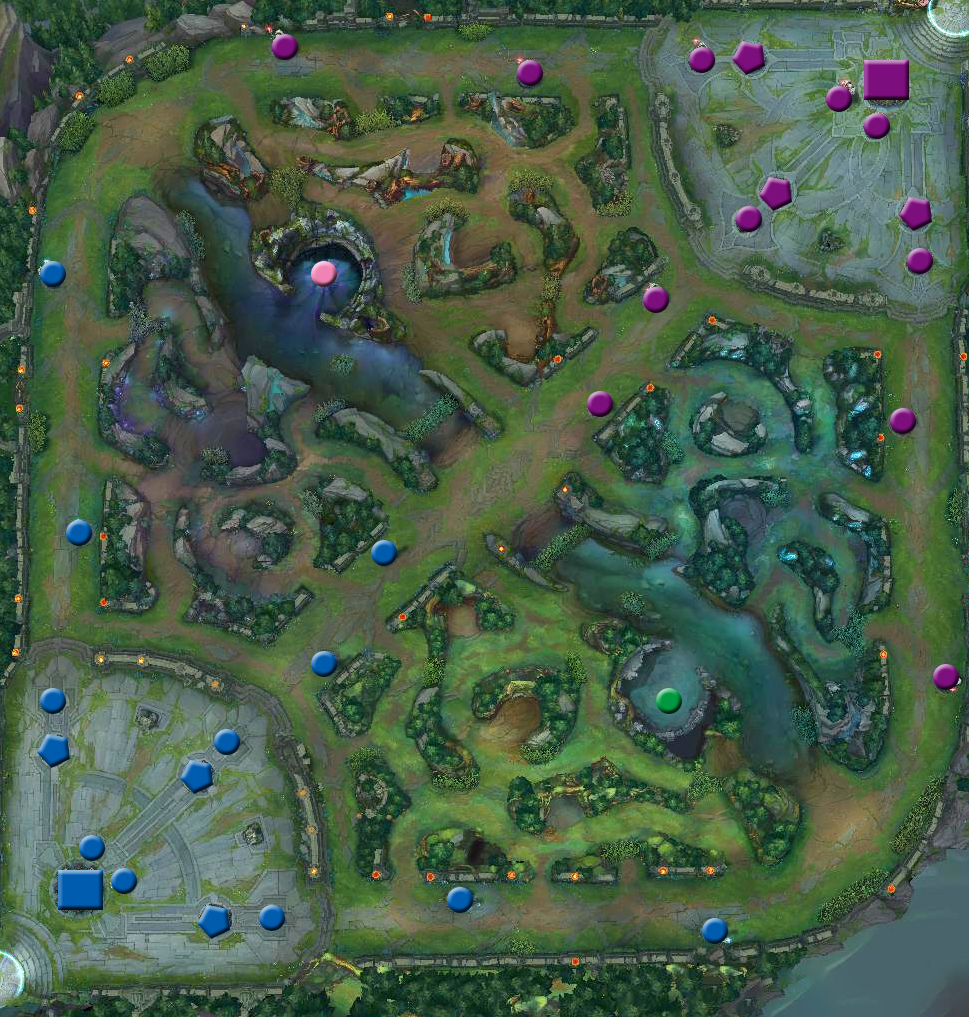
\includegraphics[width=0.5\textwidth]{img/lolmap.jpg}
  \caption{League of Legends map~\cite{lolmap}}\label{fig:lolmap}
\end{figure}

The map, seen in \Cref{fig:lolmap}, consists of three lanes, \emph{top}, \emph{middle} and \emph{bottom} which connects the two bases. The blue and purple colours represent the blue and purple teams' respective structures. Circles are turrets, pentagons are inhibitors and squares are nexuses. The green circle is the dragon and the pink circle is the baron.

\begin{table}[!h]
  \begin{tabular}{l p{13cm}}
    \textbf{Nexus}: & Spawn \emph{creeps}, which are small monsters with low damage and health, that walks along the lanes toward the opposing base. Killing these creeps award gold and experience. When destroyed the game ends, making the destroying team the winners\\
    \textbf{Inhibitor}: &  When destroyed, the destroying teams minions become stronger on that lane\\
    \textbf{Turret}: & A defensive structure, which fires at nearby enemies\\
    \textbf{Jungle}: & Area between the lanes which hosts stronger monsters that award gold and experience\\
  \end{tabular}
\end{table}

The creeps that are spawned by the nexuses walks toward the opposing teams base, which means they will meet in the middle, where the majority of the fighting will take place. When the inhibitor is destroyed, the destroying teams minions become stronger on the given lane where it was destroyed. Lastly, killing the dragon awards the killing team with a team wide buff that increases the strength of the champions, and killing the baron makes the champions stronger temporarily.

Experience and gold is earned throughout the game, for the individual players, by killing monsters or opposing champions. The experience is used to improve the abilities of the champion while gold is spend purchasing items, that will make the player more powerful.

The game combines strategy, individual player skill, communication, and team play.
With a prize pool exceeding \$ 2,000,000 in the 2014 World Championships~\cite{lolprize}, the game attracts both serious and skillful players.
